\documentclass[11pt,]{article}
\usepackage{lmodern}
\usepackage{amssymb,amsmath}
\usepackage{ifxetex,ifluatex}
\usepackage{fixltx2e} % provides \textsubscript
\ifnum 0\ifxetex 1\fi\ifluatex 1\fi=0 % if pdftex
  \usepackage[T1]{fontenc}
  \usepackage[utf8]{inputenc}
\else % if luatex or xelatex
  \ifxetex
    \usepackage{mathspec}
  \else
    \usepackage{fontspec}
  \fi
  \defaultfontfeatures{Ligatures=TeX,Scale=MatchLowercase}
\fi
% use upquote if available, for straight quotes in verbatim environments
\IfFileExists{upquote.sty}{\usepackage{upquote}}{}
% use microtype if available
\IfFileExists{microtype.sty}{%
\usepackage{microtype}
\UseMicrotypeSet[protrusion]{basicmath} % disable protrusion for tt fonts
}{}
\usepackage[margin=1in]{geometry}
\usepackage{hyperref}
\PassOptionsToPackage{usenames,dvipsnames}{color} % color is loaded by hyperref
\hypersetup{unicode=true,
            pdftitle={Data Visualization},
            colorlinks=true,
            linkcolor=Maroon,
            citecolor=Blue,
            urlcolor=blue,
            breaklinks=true}
\urlstyle{same}  % don't use monospace font for urls
\usepackage{color}
\usepackage{fancyvrb}
\newcommand{\VerbBar}{|}
\newcommand{\VERB}{\Verb[commandchars=\\\{\}]}
\DefineVerbatimEnvironment{Highlighting}{Verbatim}{commandchars=\\\{\}}
% Add ',fontsize=\small' for more characters per line
\usepackage{framed}
\definecolor{shadecolor}{RGB}{248,248,248}
\newenvironment{Shaded}{\begin{snugshade}}{\end{snugshade}}
\newcommand{\AlertTok}[1]{\textcolor[rgb]{0.94,0.16,0.16}{#1}}
\newcommand{\AnnotationTok}[1]{\textcolor[rgb]{0.56,0.35,0.01}{\textbf{\textit{#1}}}}
\newcommand{\AttributeTok}[1]{\textcolor[rgb]{0.77,0.63,0.00}{#1}}
\newcommand{\BaseNTok}[1]{\textcolor[rgb]{0.00,0.00,0.81}{#1}}
\newcommand{\BuiltInTok}[1]{#1}
\newcommand{\CharTok}[1]{\textcolor[rgb]{0.31,0.60,0.02}{#1}}
\newcommand{\CommentTok}[1]{\textcolor[rgb]{0.56,0.35,0.01}{\textit{#1}}}
\newcommand{\CommentVarTok}[1]{\textcolor[rgb]{0.56,0.35,0.01}{\textbf{\textit{#1}}}}
\newcommand{\ConstantTok}[1]{\textcolor[rgb]{0.00,0.00,0.00}{#1}}
\newcommand{\ControlFlowTok}[1]{\textcolor[rgb]{0.13,0.29,0.53}{\textbf{#1}}}
\newcommand{\DataTypeTok}[1]{\textcolor[rgb]{0.13,0.29,0.53}{#1}}
\newcommand{\DecValTok}[1]{\textcolor[rgb]{0.00,0.00,0.81}{#1}}
\newcommand{\DocumentationTok}[1]{\textcolor[rgb]{0.56,0.35,0.01}{\textbf{\textit{#1}}}}
\newcommand{\ErrorTok}[1]{\textcolor[rgb]{0.64,0.00,0.00}{\textbf{#1}}}
\newcommand{\ExtensionTok}[1]{#1}
\newcommand{\FloatTok}[1]{\textcolor[rgb]{0.00,0.00,0.81}{#1}}
\newcommand{\FunctionTok}[1]{\textcolor[rgb]{0.00,0.00,0.00}{#1}}
\newcommand{\ImportTok}[1]{#1}
\newcommand{\InformationTok}[1]{\textcolor[rgb]{0.56,0.35,0.01}{\textbf{\textit{#1}}}}
\newcommand{\KeywordTok}[1]{\textcolor[rgb]{0.13,0.29,0.53}{\textbf{#1}}}
\newcommand{\NormalTok}[1]{#1}
\newcommand{\OperatorTok}[1]{\textcolor[rgb]{0.81,0.36,0.00}{\textbf{#1}}}
\newcommand{\OtherTok}[1]{\textcolor[rgb]{0.56,0.35,0.01}{#1}}
\newcommand{\PreprocessorTok}[1]{\textcolor[rgb]{0.56,0.35,0.01}{\textit{#1}}}
\newcommand{\RegionMarkerTok}[1]{#1}
\newcommand{\SpecialCharTok}[1]{\textcolor[rgb]{0.00,0.00,0.00}{#1}}
\newcommand{\SpecialStringTok}[1]{\textcolor[rgb]{0.31,0.60,0.02}{#1}}
\newcommand{\StringTok}[1]{\textcolor[rgb]{0.31,0.60,0.02}{#1}}
\newcommand{\VariableTok}[1]{\textcolor[rgb]{0.00,0.00,0.00}{#1}}
\newcommand{\VerbatimStringTok}[1]{\textcolor[rgb]{0.31,0.60,0.02}{#1}}
\newcommand{\WarningTok}[1]{\textcolor[rgb]{0.56,0.35,0.01}{\textbf{\textit{#1}}}}
\usepackage{graphicx,grffile}
\makeatletter
\def\maxwidth{\ifdim\Gin@nat@width>\linewidth\linewidth\else\Gin@nat@width\fi}
\def\maxheight{\ifdim\Gin@nat@height>\textheight\textheight\else\Gin@nat@height\fi}
\makeatother
% Scale images if necessary, so that they will not overflow the page
% margins by default, and it is still possible to overwrite the defaults
% using explicit options in \includegraphics[width, height, ...]{}
\setkeys{Gin}{width=\maxwidth,height=\maxheight,keepaspectratio}
\IfFileExists{parskip.sty}{%
\usepackage{parskip}
}{% else
\setlength{\parindent}{0pt}
\setlength{\parskip}{6pt plus 2pt minus 1pt}
}
\setlength{\emergencystretch}{3em}  % prevent overfull lines
\providecommand{\tightlist}{%
  \setlength{\itemsep}{0pt}\setlength{\parskip}{0pt}}
\setcounter{secnumdepth}{5}
% Redefines (sub)paragraphs to behave more like sections
\ifx\paragraph\undefined\else
\let\oldparagraph\paragraph
\renewcommand{\paragraph}[1]{\oldparagraph{#1}\mbox{}}
\fi
\ifx\subparagraph\undefined\else
\let\oldsubparagraph\subparagraph
\renewcommand{\subparagraph}[1]{\oldsubparagraph{#1}\mbox{}}
\fi

%%% Use protect on footnotes to avoid problems with footnotes in titles
\let\rmarkdownfootnote\footnote%
\def\footnote{\protect\rmarkdownfootnote}

%%% Change title format to be more compact
\usepackage{titling}

% Create subtitle command for use in maketitle
\providecommand{\subtitle}[1]{
  \posttitle{
    \begin{center}\large#1\end{center}
    }
}

\setlength{\droptitle}{-2em}

  \title{Data Visualization}
    \pretitle{\vspace{\droptitle}\centering\huge}
  \posttitle{\par}
    \author{}
    \preauthor{}\postauthor{}
      \predate{\centering\large\emph}
  \postdate{\par}
    \date{May 14, 2019}


\begin{document}
\maketitle

{
\hypersetup{linkcolor=black}
\setcounter{tocdepth}{2}
\tableofcontents
}
\begin{quote}
\hypertarget{learning-objectives}{%
\subsection{Learning Objectives}\label{learning-objectives}}

\begin{itemize}
\tightlist
\item
  Grammar of graphics concepts (geoms, aesthetics)
\item
  Advanced plots (scales, facets, themes)
\item
  Writing images (and other things) to file
\end{itemize}
\end{quote}

\hypertarget{basic-plots-in-r}{%
\section{Basic plots in R}\label{basic-plots-in-r}}

When we are working with large sets of numbers it can be useful to
display that information graphically. R has a number of built-in tools
for basic graph types such as hisotgrams, scatter plots, bar charts,
boxplots and much \href{http://www.statmethods.net/graphs/}{more}. We'll
test a few of these out here on the \texttt{cats} data.

\begin{Shaded}
\begin{Highlighting}[]
\KeywordTok{library}\NormalTok{(dplyr)}
\end{Highlighting}
\end{Shaded}

\begin{verbatim}
## 
## Attaching package: 'dplyr'
\end{verbatim}

\begin{verbatim}
## The following objects are masked from 'package:stats':
## 
##     filter, lag
\end{verbatim}

\begin{verbatim}
## The following objects are masked from 'package:base':
## 
##     intersect, setdiff, setequal, union
\end{verbatim}

\begin{Shaded}
\begin{Highlighting}[]
\NormalTok{cats <-}\StringTok{ }\KeywordTok{read.csv}\NormalTok{(}\StringTok{"data/herding-cats.csv"}\NormalTok{)}
\end{Highlighting}
\end{Shaded}

\hypertarget{scatterplot}{%
\subsection{Scatterplot}\label{scatterplot}}

Let's start with a \textbf{scatterplot}. A scatter plot provides a
graphical view of the relationship between two sets of numbers.

Let's make a scatterplot of birth weight by mother's age.

\begin{Shaded}
\begin{Highlighting}[]
\KeywordTok{plot}\NormalTok{(}\DataTypeTok{x =}\NormalTok{ cats}\OperatorTok{$}\NormalTok{age, }\DataTypeTok{y =}\NormalTok{ cats}\OperatorTok{$}\NormalTok{weight)}
\end{Highlighting}
\end{Shaded}

\begin{center}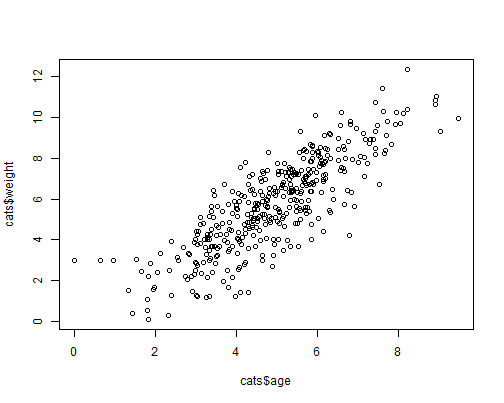
\includegraphics{06-data-visualization_files/figure-latex/scatter-plot1-1} \end{center}

Each point represents a row in our dataset. The value on the x-axis is
the mother's age and the values on the y-axis correspond to the birth
weight for the infant. For any plot you can customize many features of
your graphs (fonts, colors, axes, titles) through
\href{http://www.statmethods.net/advgraphs/parameters.html}{graphic
options}

\hypertarget{advanced-figures-ggplot2}{%
\section{\texorpdfstring{Advanced figures
(\texttt{ggplot2})}{Advanced figures (ggplot2)}}\label{advanced-figures-ggplot2}}

More recently, R users have moved away from base graphic options and
towards a plotting package called \texttt{ggplot2} that adds a lot of
functionality to the basic plots seen above. The syntax is different but
it's extremely powerful and flexible. We can start by re-creating some
of the above plots but using ggplot functions to get a feel for the
syntax.

\begin{Shaded}
\begin{Highlighting}[]
\KeywordTok{install.packages}\NormalTok{(}\StringTok{"ggplot2"}\NormalTok{)}
\end{Highlighting}
\end{Shaded}

Load the \texttt{ggplot2} package.

\begin{Shaded}
\begin{Highlighting}[]
\KeywordTok{library}\NormalTok{(ggplot2)}
\end{Highlighting}
\end{Shaded}

The \texttt{ggplot()} function is used to initialize the basic graph
structure, then we add to it. The basic idea is that you specify
different parts of the plot, and add them together using the + operator.

We will start with a blank plot and will find that you will get an
error, because you need to add layers.

\begin{Shaded}
\begin{Highlighting}[]
\KeywordTok{ggplot}\NormalTok{(cats)}
\end{Highlighting}
\end{Shaded}

\begin{center}
\includegraphics{06-data-visualization_files/figure-latex/unnamed-chunk-1-1} \end{center}

Geometric objects are the actual marks we put on a plot. Examples
include:

\begin{itemize}
\tightlist
\item
  points (geom\_point, for scatter plots, dot plots, etc)
\item
  lines (geom\_line, for time series, trend lines, etc)
\item
  boxplot (geom\_boxplot, for, well, boxplots!)
\end{itemize}

A plot must have at least one geom; there is no upper limit. You can add
a geom to a plot using the \texttt{+} operator.

\begin{Shaded}
\begin{Highlighting}[]
\KeywordTok{ggplot}\NormalTok{(cats) }\OperatorTok{+}
\StringTok{    }\KeywordTok{geom_point}\NormalTok{()}
\end{Highlighting}
\end{Shaded}

Each type of geom usually has a required set of aesthetics to be set,
and usually accepts only a subset of all aesthetics --refer to the geom
help pages to see what mappings each geom accepts. Aesthetic mappings
are set with the \texttt{aes()} function.

Examples include:

\begin{itemize}
\tightlist
\item
  position (i.e., on the x and y axes)
\item
  color (``outside'' color)
\item
  fill (``inside'' color) shape (of points)
\item
  linetype
\item
  size
\end{itemize}

To start, we will add position for the x- and y-axis since geom\_point
requires mappings for x and y, all others are optional.

\begin{Shaded}
\begin{Highlighting}[]
\KeywordTok{ggplot}\NormalTok{(cats) }\OperatorTok{+}
\StringTok{    }\KeywordTok{geom_point}\NormalTok{(}\KeywordTok{aes}\NormalTok{(}\DataTypeTok{x =}\NormalTok{ age, }\DataTypeTok{y =}\NormalTok{ weight),}
               \DataTypeTok{color =} \StringTok{"red"}\NormalTok{,}
               \DataTypeTok{alpha =} \FloatTok{0.5}\NormalTok{,}
               \DataTypeTok{shape =} \DecValTok{1}\NormalTok{,}
               \DataTypeTok{size =} \DecValTok{3}\NormalTok{)}
\end{Highlighting}
\end{Shaded}

\begin{center}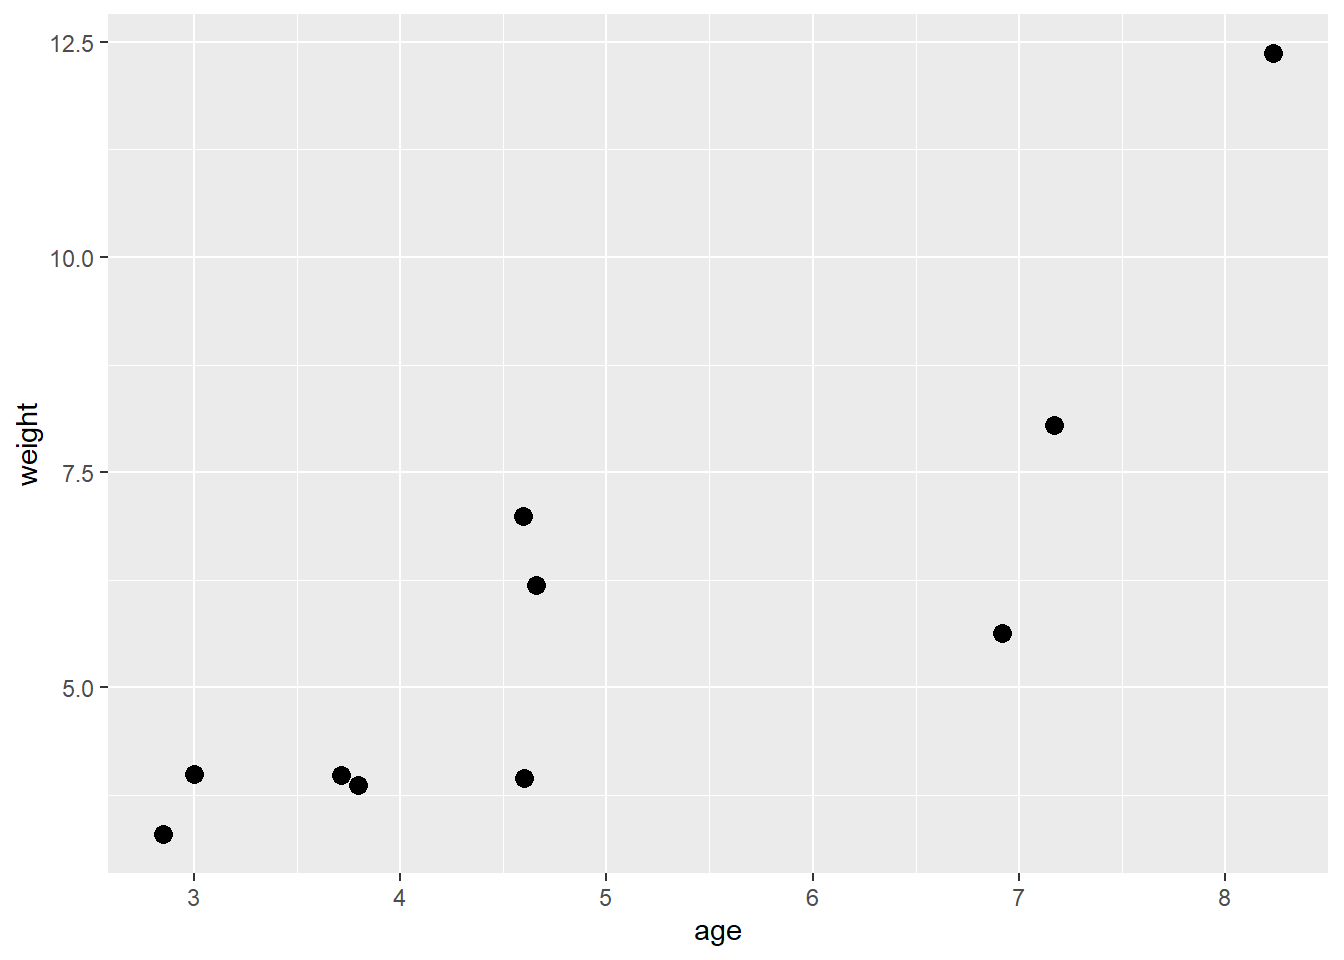
\includegraphics{06-data-visualization_files/figure-latex/unnamed-chunk-3-1} \end{center}

\#\#\#Scales

Scales control the mapping between data and aesthetics.

\begin{Shaded}
\begin{Highlighting}[]
\KeywordTok{ggplot}\NormalTok{(cats) }\OperatorTok{+}
\StringTok{    }\KeywordTok{geom_point}\NormalTok{(}\KeywordTok{aes}\NormalTok{(}\DataTypeTok{x =}\NormalTok{ age, }\DataTypeTok{y =}\NormalTok{ weight)) }\OperatorTok{+}
\StringTok{    }\KeywordTok{scale_x_continuous}\NormalTok{(}\DataTypeTok{name =} \StringTok{"Age"}\NormalTok{,}
                       \DataTypeTok{breaks =} \KeywordTok{c}\NormalTok{(}\DecValTok{1}\NormalTok{, }\DecValTok{2}\NormalTok{, }\DecValTok{3}\NormalTok{),}
                       \DataTypeTok{limits =} \KeywordTok{c}\NormalTok{(}\OperatorTok{-}\DecValTok{5}\NormalTok{, }\DecValTok{15}\NormalTok{)) }\OperatorTok{+}
\StringTok{    }\KeywordTok{scale_y_continuous}\NormalTok{(}\StringTok{"Weight"}\NormalTok{, }\DataTypeTok{trans =} \StringTok{"log"}\NormalTok{) }\OperatorTok{+}\StringTok{ }
\StringTok{    }\KeywordTok{ggtitle}\NormalTok{(}\DataTypeTok{label =} \StringTok{"Scatterplot"}\NormalTok{)}
\end{Highlighting}
\end{Shaded}

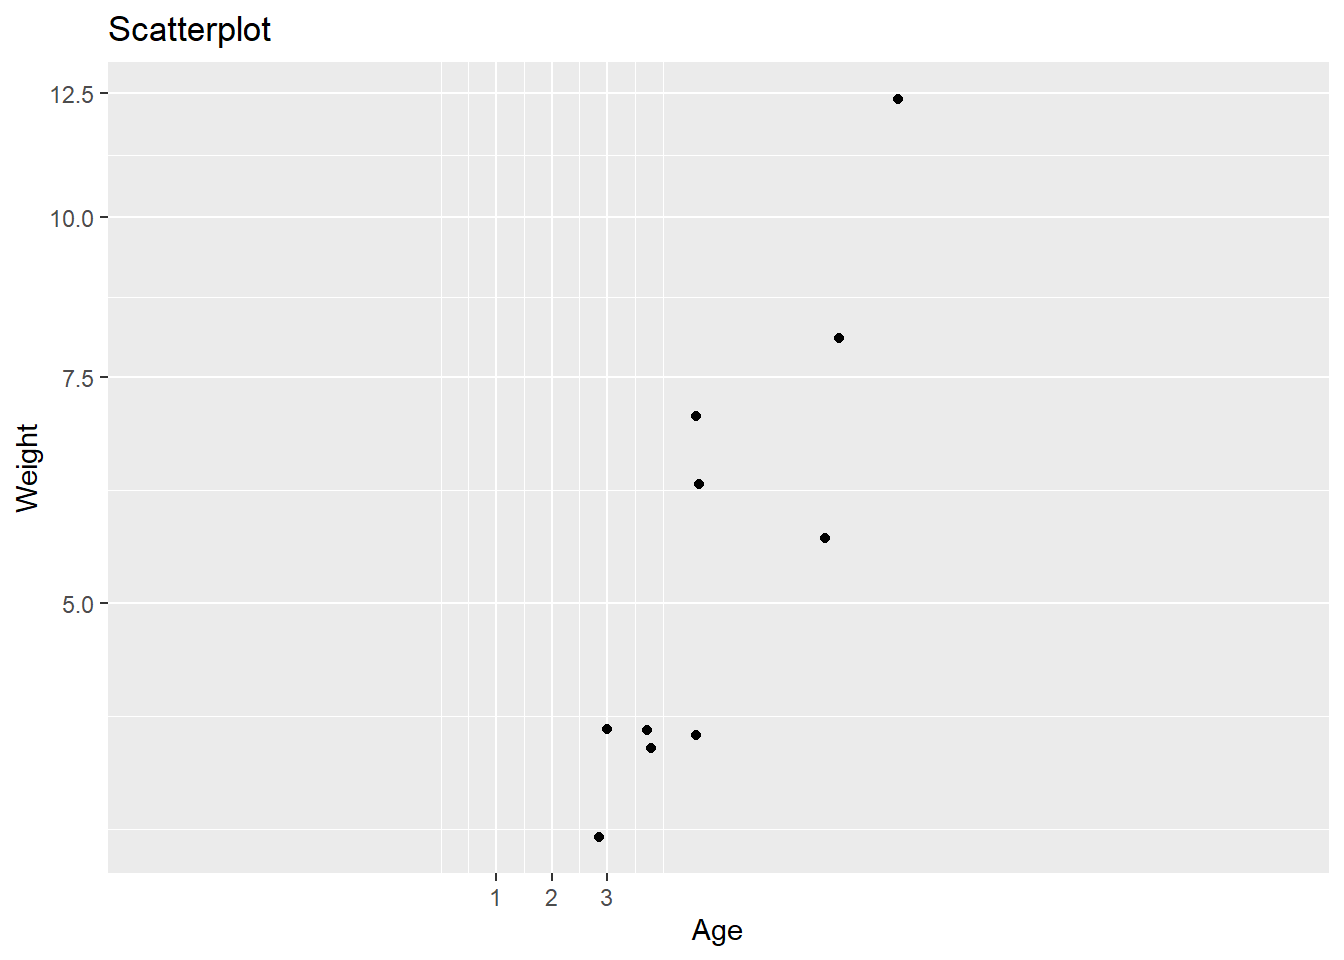
\includegraphics{06-data-visualization_files/figure-latex/unnamed-chunk-4-1.pdf}

\#\#\#Themes

The ggplot2 theme system handles non-data plot elements such as:

\begin{itemize}
\tightlist
\item
  Axis labels
\item
  Plot background
\item
  Facet label backround
\item
  Legend appearance
\end{itemize}

There are built-in themes we can use, or we can adjust specific
elements. We can add additional aesthetics by mapping them to other
variables in our dataframe. For example, the color of the boxplots will
reflect low birth weight.

\begin{Shaded}
\begin{Highlighting}[]
\KeywordTok{ggplot}\NormalTok{(cats) }\OperatorTok{+}
\StringTok{    }\KeywordTok{geom_point}\NormalTok{(}\KeywordTok{aes}\NormalTok{(}\DataTypeTok{x =}\NormalTok{ age, }\DataTypeTok{y =}\NormalTok{ weight)) }\OperatorTok{+}
\StringTok{    }\KeywordTok{theme_bw}\NormalTok{()}
\end{Highlighting}
\end{Shaded}

\begin{center}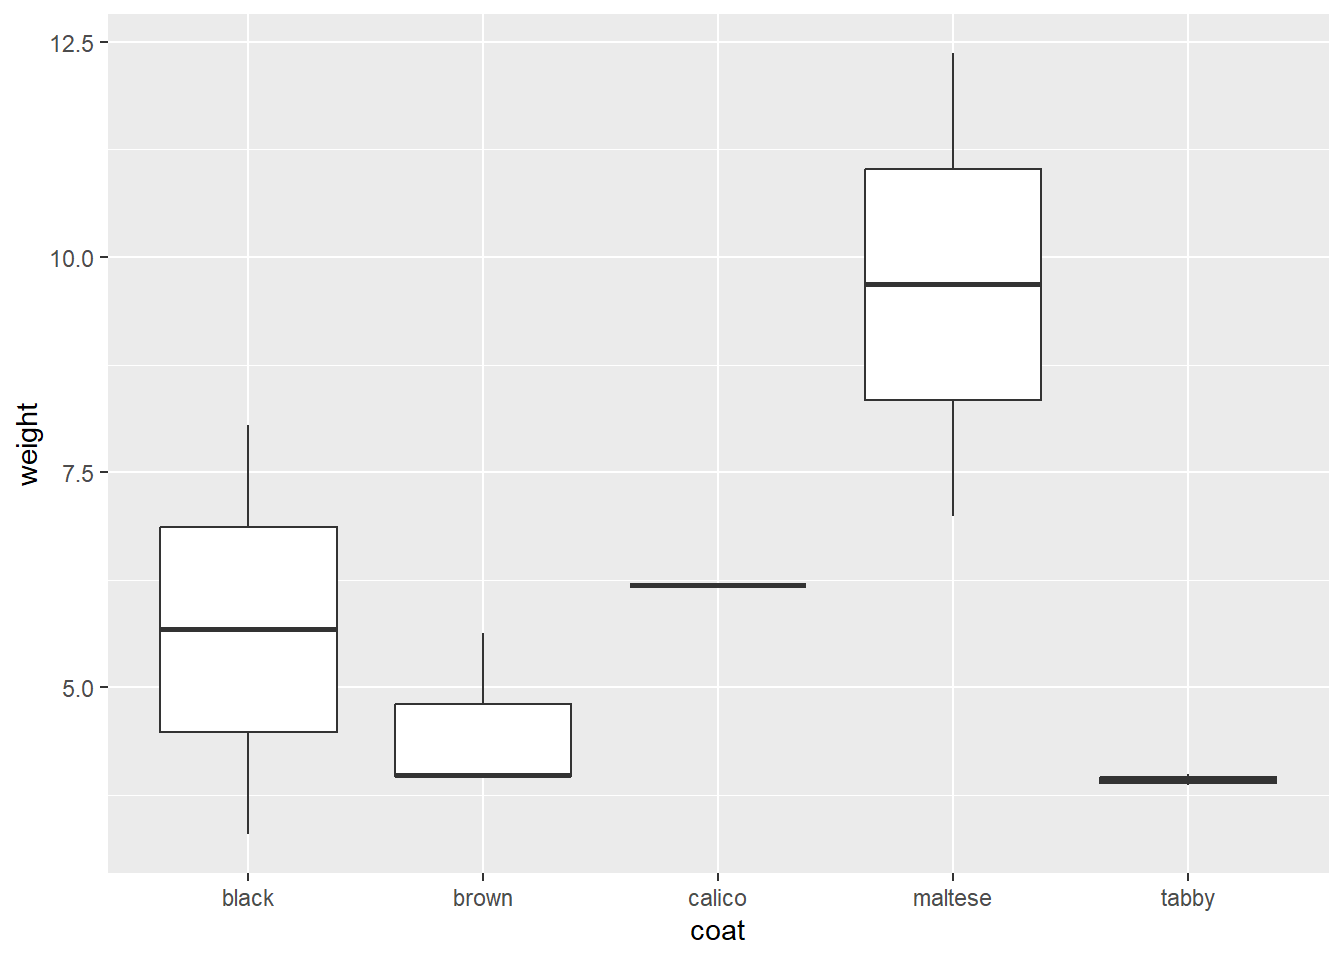
\includegraphics{06-data-visualization_files/figure-latex/unnamed-chunk-5-1} \end{center}

\#\#\#Facets

Facets display subsets of the dataset in different panels. Let's use the
\texttt{facet\_grid} function to lay out panels in a grid. Each panel
will have the same geometric objects.

\begin{Shaded}
\begin{Highlighting}[]
\KeywordTok{ggplot}\NormalTok{(cats) }\OperatorTok{+}
\StringTok{    }\KeywordTok{geom_point}\NormalTok{(}\KeywordTok{aes}\NormalTok{(}\DataTypeTok{x =}\NormalTok{ age, }\DataTypeTok{y =}\NormalTok{ weight)) }\OperatorTok{+}
\StringTok{    }\KeywordTok{xlab}\NormalTok{(}\StringTok{"Mother's age"}\NormalTok{) }\OperatorTok{+}
\StringTok{    }\KeywordTok{ylab}\NormalTok{(}\StringTok{"Birth weight"}\NormalTok{) }\OperatorTok{+}
\StringTok{    }\KeywordTok{facet_grid}\NormalTok{(. }\OperatorTok{~}\StringTok{ }\NormalTok{coat) }\OperatorTok{+}
\StringTok{    }\KeywordTok{theme_linedraw}\NormalTok{()}
\end{Highlighting}
\end{Shaded}

\textbackslash{}begin\{center\}\includegraphics{06-data-visualization_files/figure-latex/}-1\}
\textbackslash{}end\{center\}

Here we have two panels one for each factor level of \texttt{coat}. The
panels are layed out in columns because the expression
\texttt{.\ \textasciitilde{}\ coat}

\#\#\#Writing figures to file

There are two ways in which figures and plots can be output to a file
(rather than simply displaying on screen).

The first (and easiest) is to export directly from the RStudio `Plots'
panel, by clicking on Export when the image is plotted. This will give
you the option of png or pdf and selecting the directory to which you
wish to save it to.

The second option is to use R functions in the console, allowing you the
flexibility to specify parameters to dictate the size and resolution of
the output image. Some of the more popular formats include
\texttt{pdf()}, \texttt{png}, and \texttt{svg}.

Initialize a plot that will be written directly to a file using
\texttt{pdf}, \texttt{png} etc. Within the function you will need to
specify a name for your image, and the with and height (optional). Then
create a plot using the usual functions in R. Finally, close the file
using the \texttt{dev.off()} function. There are also \texttt{bmp},
\texttt{tiff}, and \texttt{jpeg} functions, though the \texttt{jpeg}
function has proven less stable than the others.

\begin{Shaded}
\begin{Highlighting}[]
\KeywordTok{ggplot}\NormalTok{(example_data) }\OperatorTok{+}
\StringTok{  }\KeywordTok{geom_boxplot}\NormalTok{(}\KeywordTok{aes}\NormalTok{(}\DataTypeTok{x =}\NormalTok{ cit, }\DataTypeTok{y =}\NormalTok{....) }\OperatorTok{+}
\StringTok{  }\KeywordTok{ggtitle}\NormalTok{(...) }\OperatorTok{+}
\StringTok{  }\KeywordTok{xlab}\NormalTok{(...) }\OperatorTok{+}
\StringTok{  }\KeywordTok{ylab}\NormalTok{(...) }\OperatorTok{+}
\StringTok{  }\KeywordTok{theme}\NormalTok{(}\DataTypeTok{panel.grid.major =} \KeywordTok{element_line}\NormalTok{(...),}
          \DataTypeTok{axis.text.x =} \KeywordTok{element_text}\NormalTok{(...),}
          \DataTypeTok{axis.title =} \KeywordTok{element_text}\NormalTok{(...),}
          \DataTypeTok{axis.text =} \KeywordTok{element_text}\NormalTok{(...)}
\end{Highlighting}
\end{Shaded}

\#\#Resources

We have only scratched the surface here. There are many plotting
features we haven't covered.

plotting in Base R:

\begin{itemize}
\tightlist
\item
  John Maindonald's
  \href{https://cran.r-project.org/doc/contrib/usingR.pdf}{Using R for
  Data Analysis and Graphics PDF}
\end{itemize}

ggplot2:

\begin{itemize}
\tightlist
\item
  \href{http://docs.ggplot2.org/}{ggplot reference site}
\item
  Winston Chang's excellent \href{http://www.cookbook-r.com}{Cookbook
  for R}
\item
  \href{http://www.amazon.com/ggplot2-Elegant-Graphics-Data-Analysis/dp/0387981403}{ggplot2:
  Elegant Graphics for Data Anaysis}
\end{itemize}

Much of the material here was adpapted from
\href{http://tutorials.iq.harvard.edu/R/Rgraphics/Rgraphics.html}{Introduction
to R graphics with ggplot2 Tutorial at IQSS}.


\end{document}
